\chapter{Alpha Wave: inhibition signal}
\label{chapter:four}
\epigraph{The electroencephalogram represents a continuous curve with continuous oscillations in which... one can distinguish larger first order waves with an average duration of 90 milliseconds...}{Berger}

This Chapter describes the experiments performed over a well-established but still mysterious EEG cognitive signal: The Berger Rhythm or Visual Occipital Alpha Waves.  An own dataset of resting subjects with and without alpha blocking is produced and the details of their generation are outlined.  Additionally, an experiment on a public Dataset is also delineated.  Conclusions and discussion are described in the last section.

\section{Introduction}

%We gather the first dataset  using the EEG EPOC Emotiv Headset and we  access the raw signals using its C++ SDK provided by the manufacturer.  The device sends wirelessly  digitalized 128 Hz sampled EEG information as discrete packets.  Every packet is numbered and the electronic impedance is constantly measured, and delivered as part of the packet information. The wireless transmitter connects to a standard RF dongle which receives the information from  14 channels and forwards it into the PC, particularly to a custom C++ EEG Datalogger program that was developed in-house.  The program is waiting passively until a new packet is received from the dongle, verifying the packet numbering and controlling that the impedance is bellow a certain level, according to the device's documentation \cite{Stopczynski2014}. 

Alpha Waves were the first signals ever spotted from the Electroencephalography.  They are regularly characterized as $10\si{Hz}$, or more broadly between the frequency band of $8$-$12$ $\si{Hz}$. They are physiologically consistent across subjects, though it has been reported inter- and intra- variations with functional cognitive implications~\cite{Haegens2014}.   Moreover, they are associated with synchronous inhibitory processes and attention shifting~\cite{c3}. They tend to be more prominent while subject's eyes are closed and appear stronger in occipital regions, around $O_1$ and $O_2$~\cite{c6,Stopczynski2014}. These waves are also called Prominent Posterior Alpha or Posterior Dominant Rhythm due to their pervasiveness in EEG~\cite{Schomer2010,Haegens2014}.

Figure~\ref{fig:alphawavessignals} shows two records of 8-channels signals.  Figure ~\ref{fig:alphawavessignals}(a) contains the registered alpha waves of a subject with their eyes open while the (b) contains the same information with their eyes closed.  The characteristic pattern of wiggles can be spotted in the latter, while their absence entails the blocking of alpha waves in the former~\cite{Basar2012}.

\begin{figure}[h!]
\centering
\subfigure[EEG signals of a relaxed healthy subject with their eyes open.]
{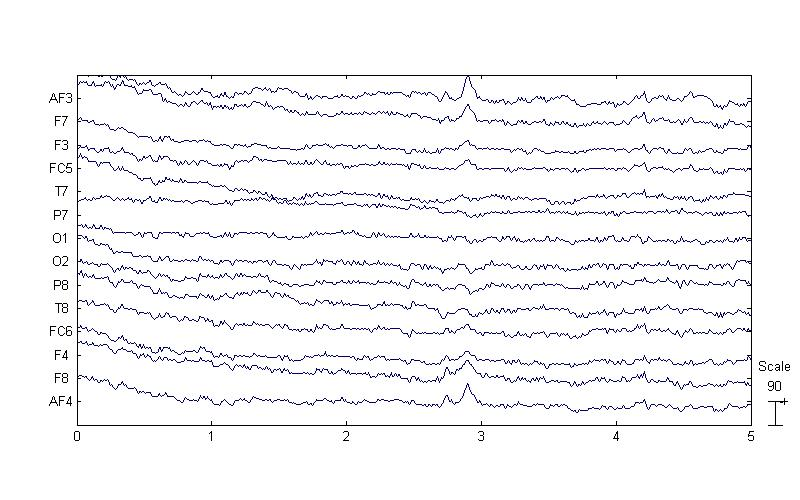
\includegraphics[height=5cm,width=7.5cm]{images/eeglab1.jpg}}
\subfigure[EEG signals of the same relaxed subject with their eyes closed. Alpha Waves wiggles can be spotted since the first second.]
{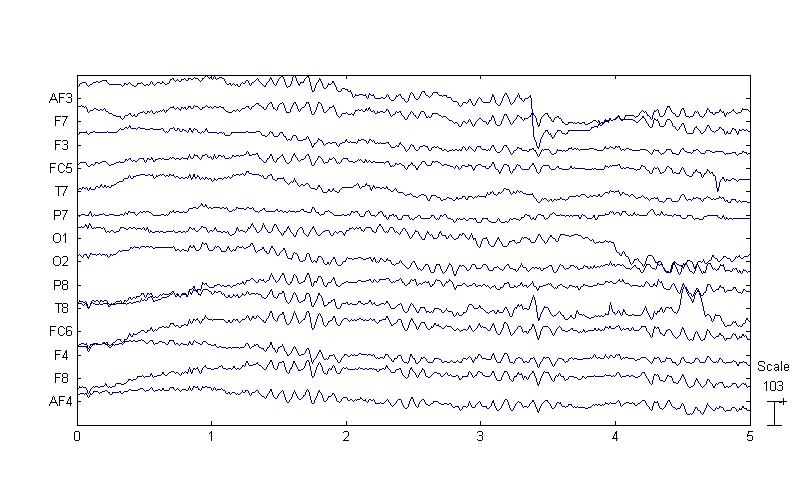
\includegraphics[height=5cm,width=7.5cm]{images/eeglab2.jpg}}
\caption[Alpha Waves Wiggles]{Five seconds of EEG signals obtained from the Emotiv EPOC device.  Fourteen channels are shown.}
\label{fig:alphawavessignals}
\end{figure}

This important rhythm is an oscillatory process.  As such, it is understood and studied in the frequency-domain.   Figure~\ref{fig:alphaspectrum} show the results of applying the Fast Fourier Transform to two different segments of $10\si{\second}$ length.  For each segment, the Power Spectral Density is calculated and their values are shown on the vertical axis.  Frequency values are shown on the horizontal axis.   On Figure (a) no particular frequency component can be spotted.  However, on Figure (b) the prevalence of the 10-\si{\hertz} alpha wave component can be observed.   
 
%As can be seen in Fig. , if we process the Drowsiness dataset with a 8-12Hz band-pass filter and calculate the average power spectral density across subjects and for each channel, we can see how clearly the value corresponding to class 2 (eyes closed) is always higher than the value for class 1 (eyes open), confirming the expected result.  This also verifies how the differentiation information is contained mostly in the frequency-domain.


%(Kamiya 1968) Neurofeedback controlling voluntarily.

\begin{figure}[h!]
\centering
\subfigure[Subject was sit, relaxed in front of the Computer Monitor with his eyes open.]
{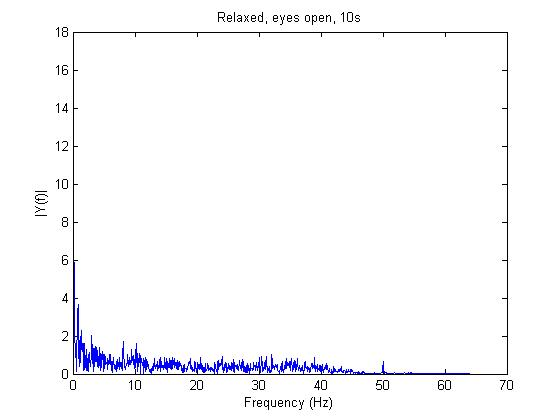
\includegraphics[height=5cm,width=7.5cm]{images/spectrumeyesopenO2.jpg}}
\subfigure[Subject was sit, relaxed in front of the Computer Monitor with his eyes closed. A strong $10 \si{Hz}$ component can be observed.]
{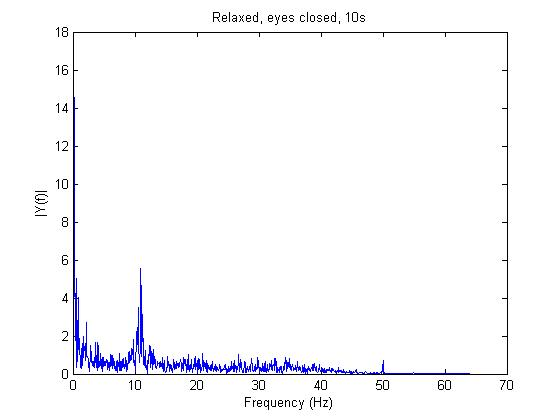
\includegraphics[height=5cm,width=7.5cm]{images/spectrumeyesclosedO2.jpg}}
\caption[Spectrum components obtained by the FFT of Alpha Waves]{Spectrum components of a $10 \si{s}$ signal segment of a subject with their eyes open. Horizontal axis shows different frequencies while the vertical axis represents the PSD.  In both diagrams a $50 \si{Hz}$ line component can be visualized.} 
\label{fig:alphaspectrum}
\end{figure}


%   \begin{figure}[thpb]
%      \centering
%      \setlength\fboxsep{0pt}
%	  \setlength\fboxrule{0.5pt}
%      \fbox{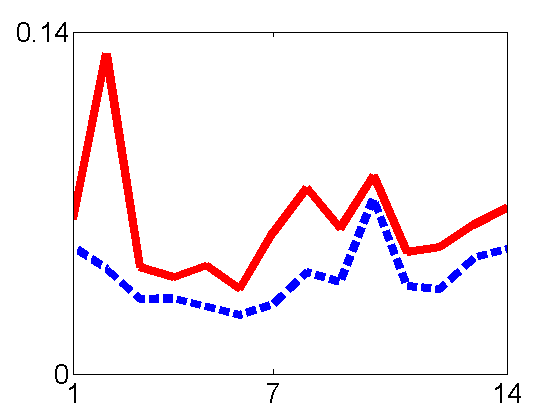
\includegraphics[width=2.5cm, height=1.8cm]{images/PSDExperiment1VsExperiment5.png}}
%      \fbox{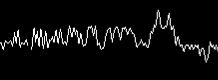
\includegraphics[width=2cm, height=1.8cm]{images/s_1_e_1_c_7_4.png}}
%      \caption[Power Spectral Density of Alpha Waves]{PSD values for every channel (x-axis) are being shown for class 1, dashed line, and class 2, solid line, for Dataset I (left). Sample EEG plot image corresponding to the subject 1 (center) for class 1 (eyes open), for the channel 7 ($ O_1 $) }
%      \label{figure1}
%   \end{figure}
   
\section{Materials and Methods}

These experiments consist in performing a binary classification of EEG signal segments between the two defined classes.  Class 2 is assigned to segments containing significant alpha waves (i.e. eyes closed), whereas class 1 identifies those where these signals are blocked (i.e. eyes open).


\subsection{Dataset I - Emotiv EPOC alpha waves own dataset}
\label{dataset1}
The first dataset is gathered using the EEG EPOC Emotiv Headset.  Although this is a commercial-grade device, it provides an acceptable price-performance ratio and it has been used to investigate basic EEG processes~\cite{Debener2012,DeVos2014}. In order to obtain the multichannel raw EEG signal, a C++ SDK library provided by the manufacturer is used and an in-house software program is developed. This device has 14 channels, and a sampling rate of 128 \si{Hz}\cite{Stopczynski2014}. Available channels are AF3, F7, F3, FC5, T7, P7, O1, O2, P8, T8,  FC6, F4, F8, AF4.  Ten healthy subjects between ages 20-50 are recruited and they accept to wear the device and to participate in the experiments.  

A 30 minutes procedure is required to adjust the headset to each user, in order to decrease the impedance on each electrode (bellow $5 \si{\kilo\ohm}$).  
This is achieved by physically adjusting the headset position over the scalp, and by embedding each electrode electrode pad in saline solution.
Once the set up is finished, each subject is instructed to sit in a relaxed position. Subsequently, she/he is commanded to watch the screen for 15 seconds, trying to avoid, as much as possible, to abruptly move its body or head.  During that time, a single-trial of 10 seconds-length window of EEG signals data is transferred to a PC and logged into standard binary files. After a 5 minutes pause, the subject is asked to close the eyes avoiding any movement while keeping the same pose for another batch of 15 seconds.  Again, 10 seconds of EEG information are transferred and logged into the PC. This finally produce a dataset of 10 subjects,  2 classes per subject, composed of 14 channels, 10-seconds length or 1280 samples per window.  These windows are further divided into 10 segments per class and per subject.

%\begin{figure}[thpb]
%\centering
%\setlength\fboxsep{0pt}
%\setlength\fboxrule{0.5pt}
%\fbox{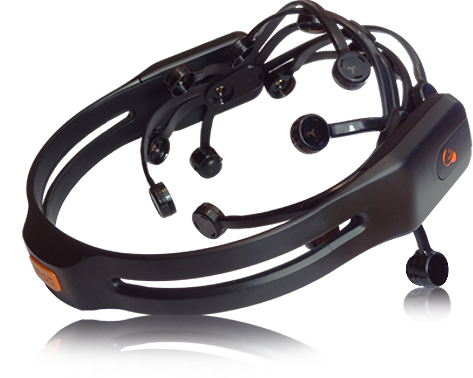
\includegraphics[width=3.5cm, height=2.5cm]{images/emotivlarge.png}}
%\fbox{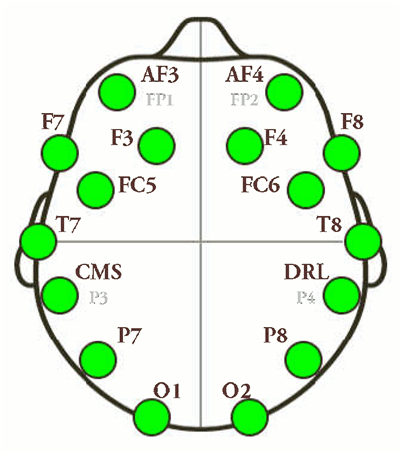
\includegraphics[width=3.5cm, height=2.5cm]{images/emotivpositions.png}}
%\fbox{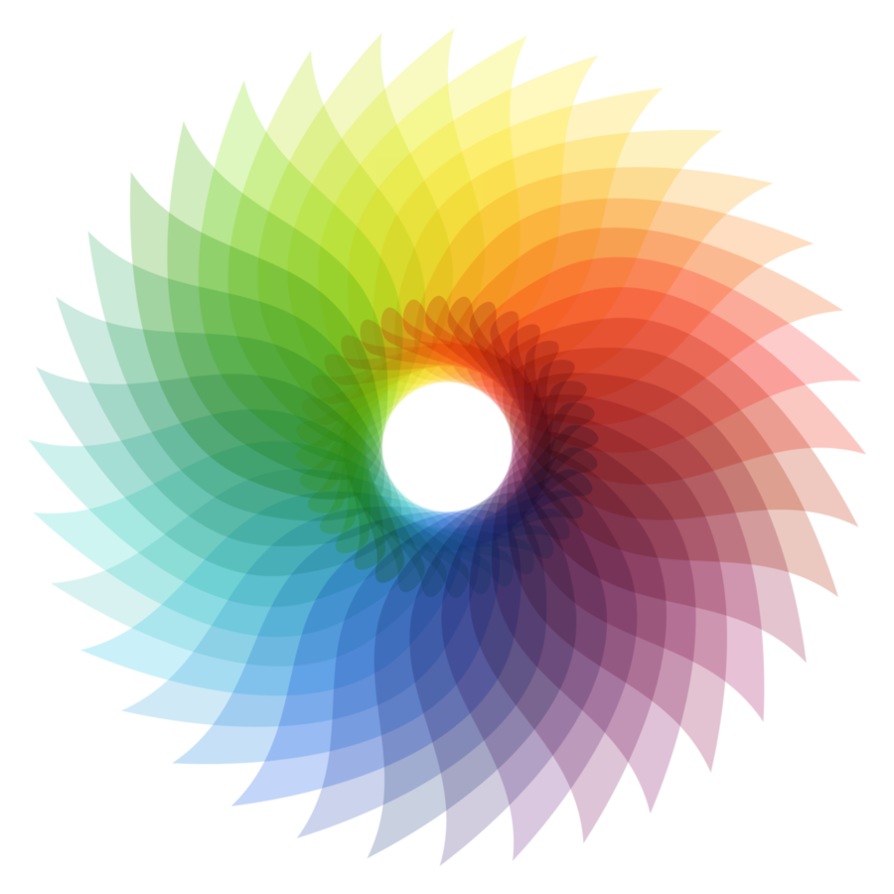
\includegraphics[width=3.5cm, height=2.5cm]{images/emotivcalibration.png}}
%\fbox{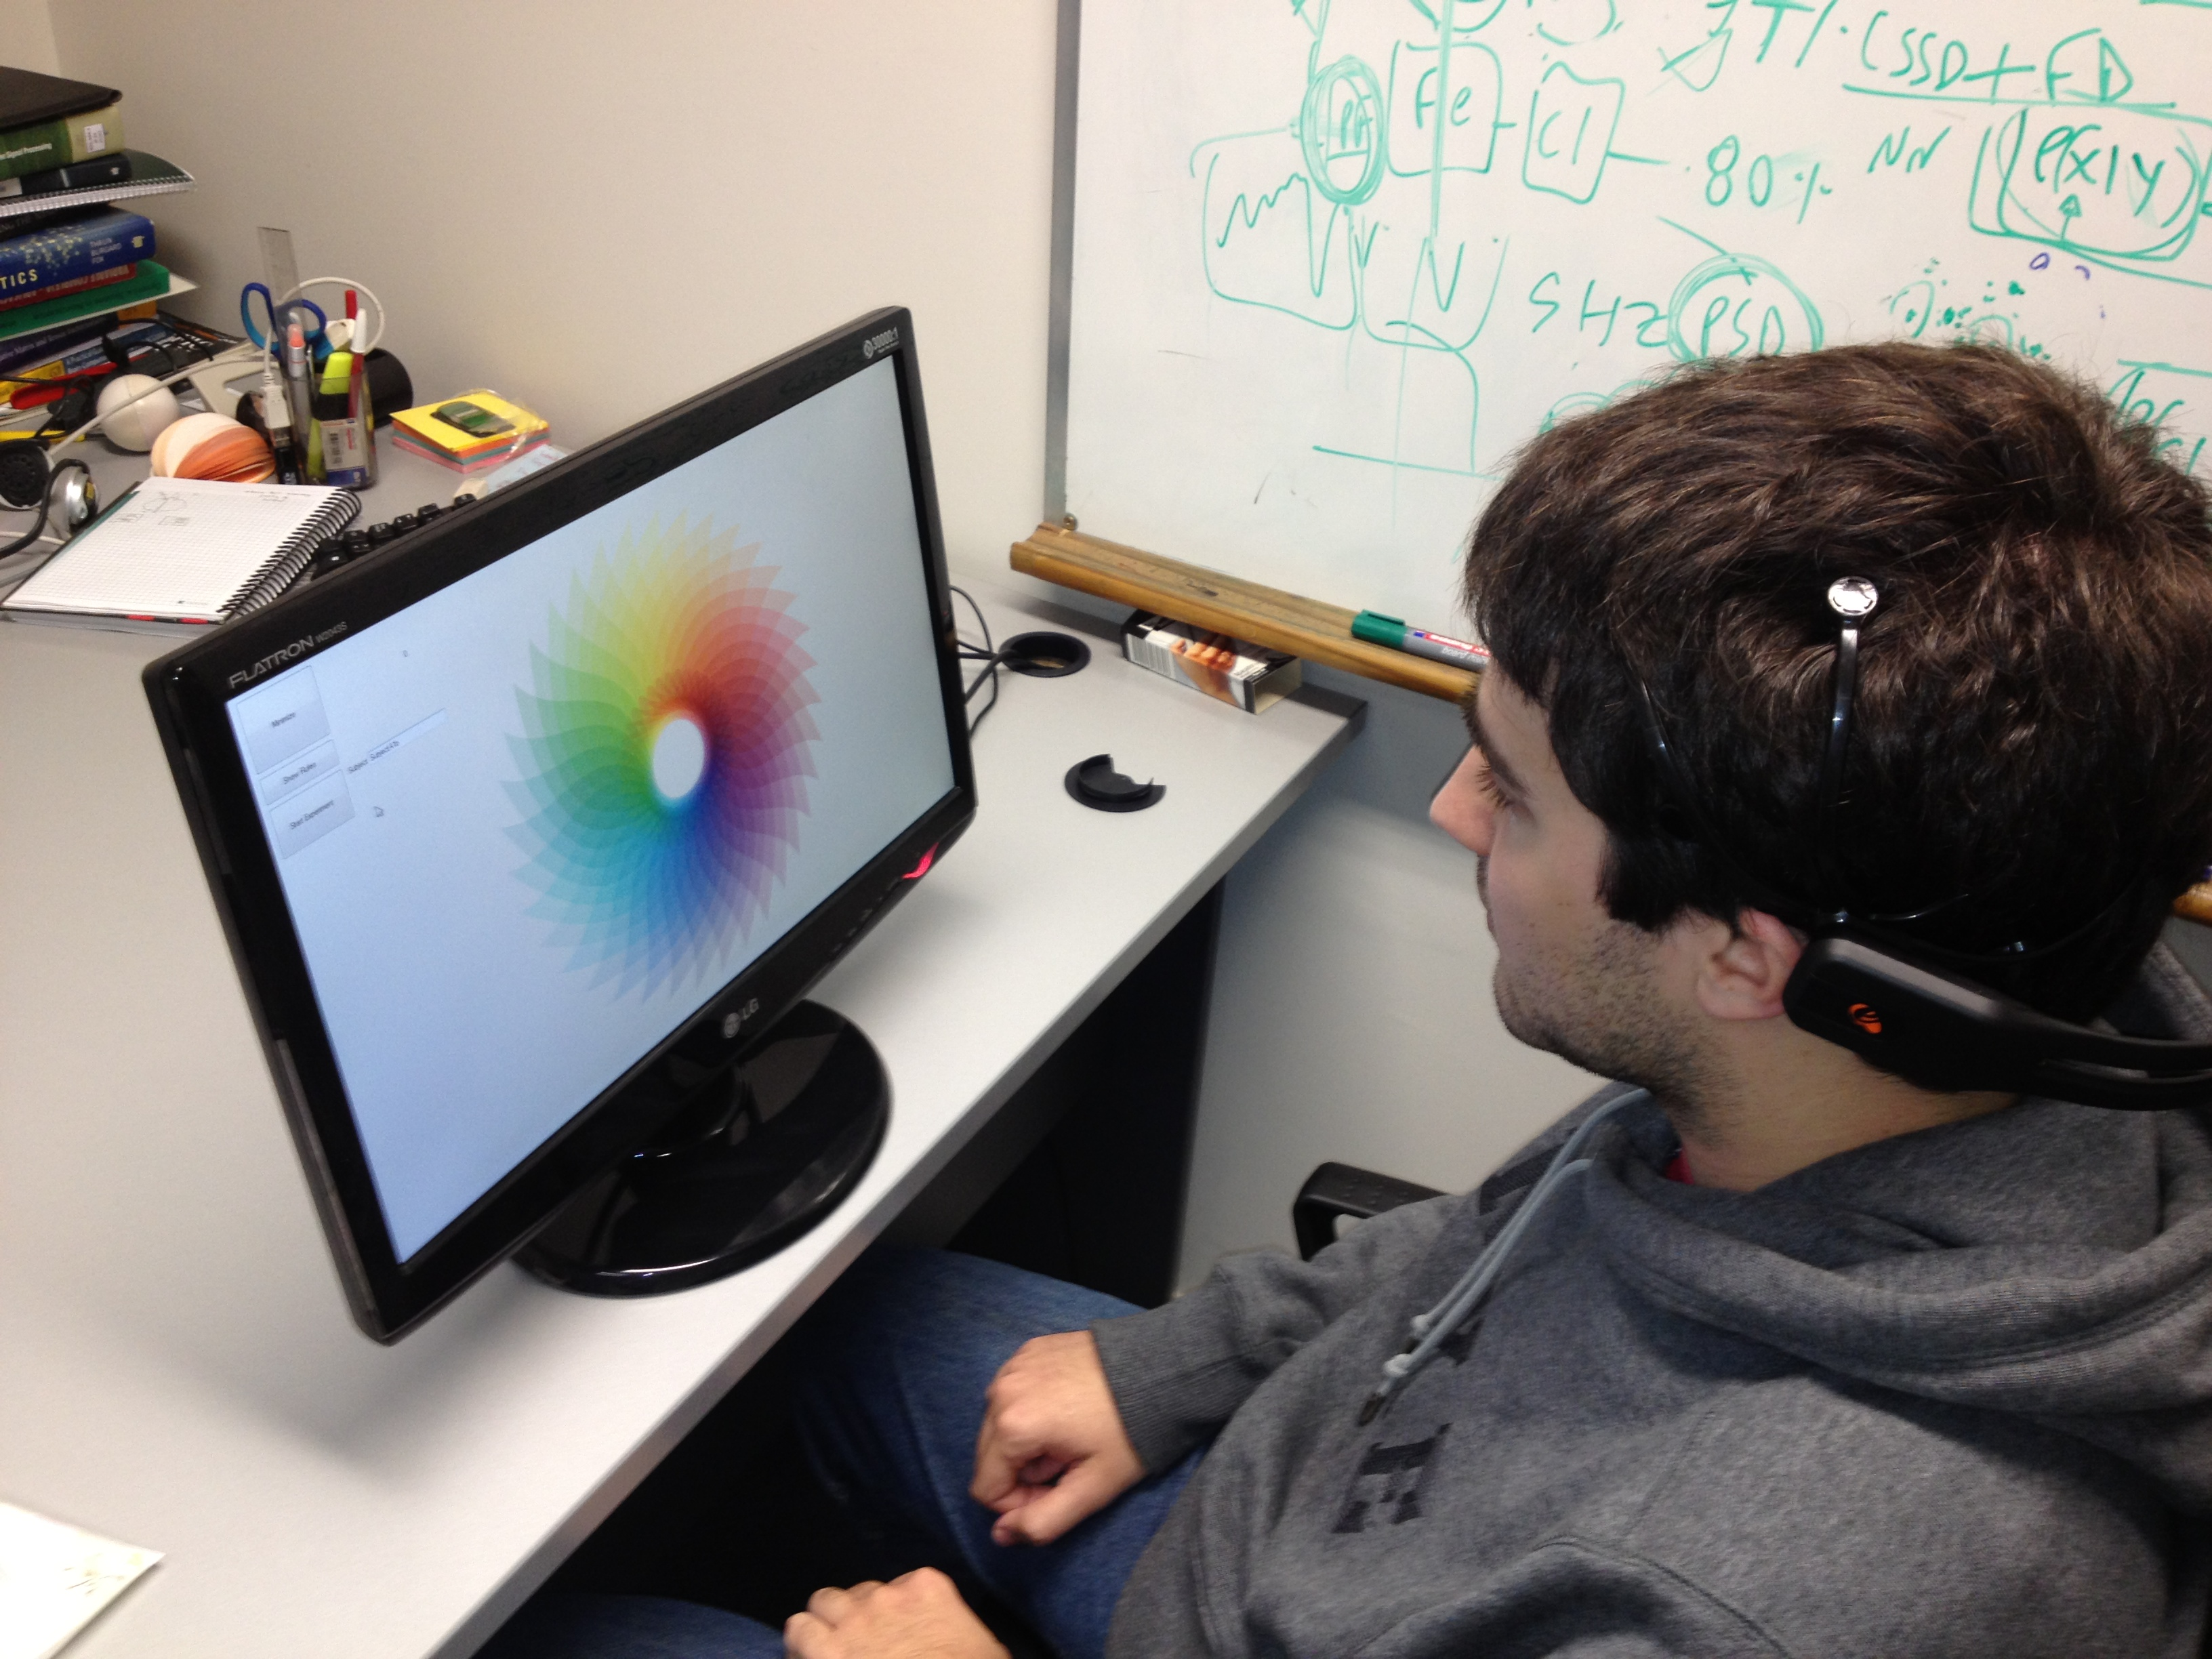
\includegraphics[width=3.5cm, height=2.5cm]{images/emotivdatasetsubject.jpg}}
%\caption[Classification Accuracy of Alpha Waves]{}
%\label{figure1}
%\end{figure}   
   
\begin{figure}[h!]
\centering
\subfigure[]
{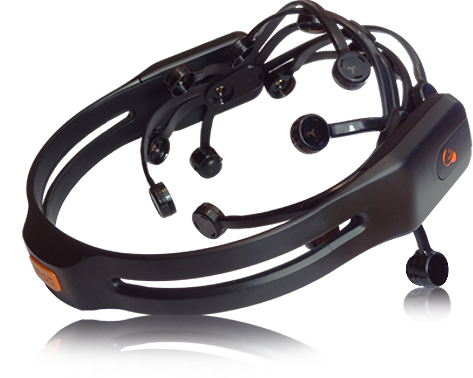
\includegraphics[width=3.5cm, height=3cm]{images/emotivlarge.png}}
\subfigure[]
{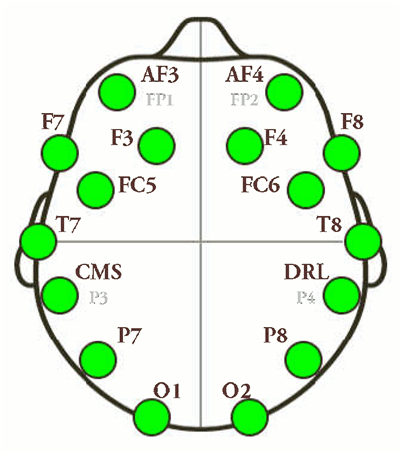
\includegraphics[width=3.5cm, height=3cm]{images/emotivpositions.png}}
\subfigure[]
{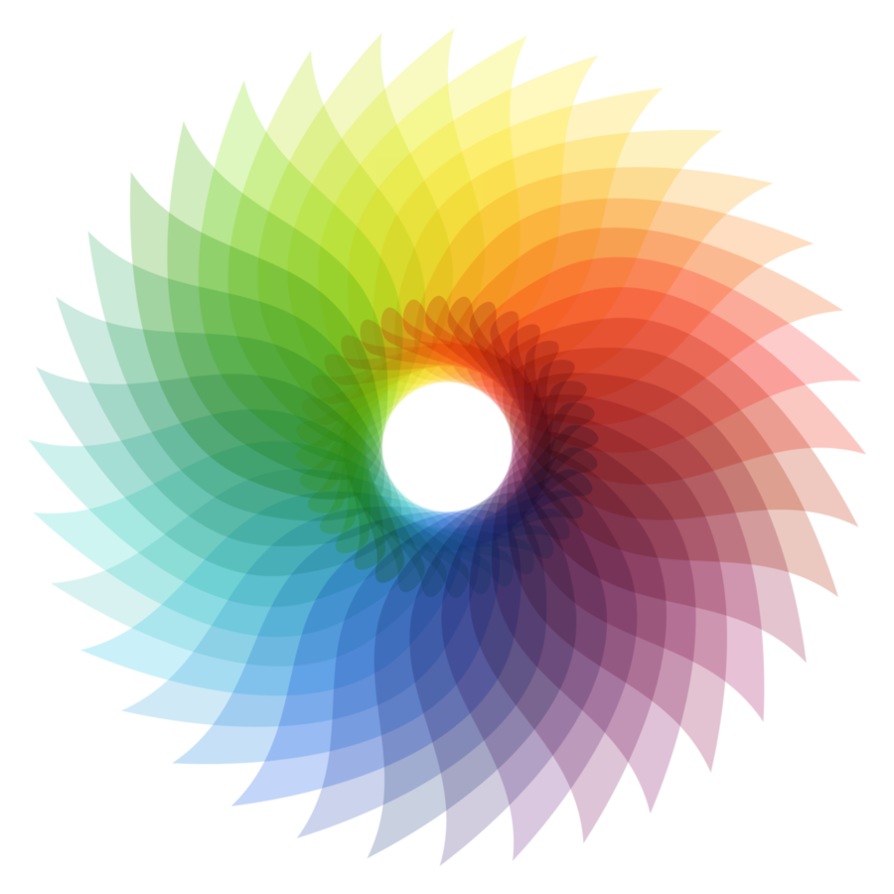
\includegraphics[width=3.5cm, height=3cm]{images/emotivcalibration.png}}
\subfigure[]
{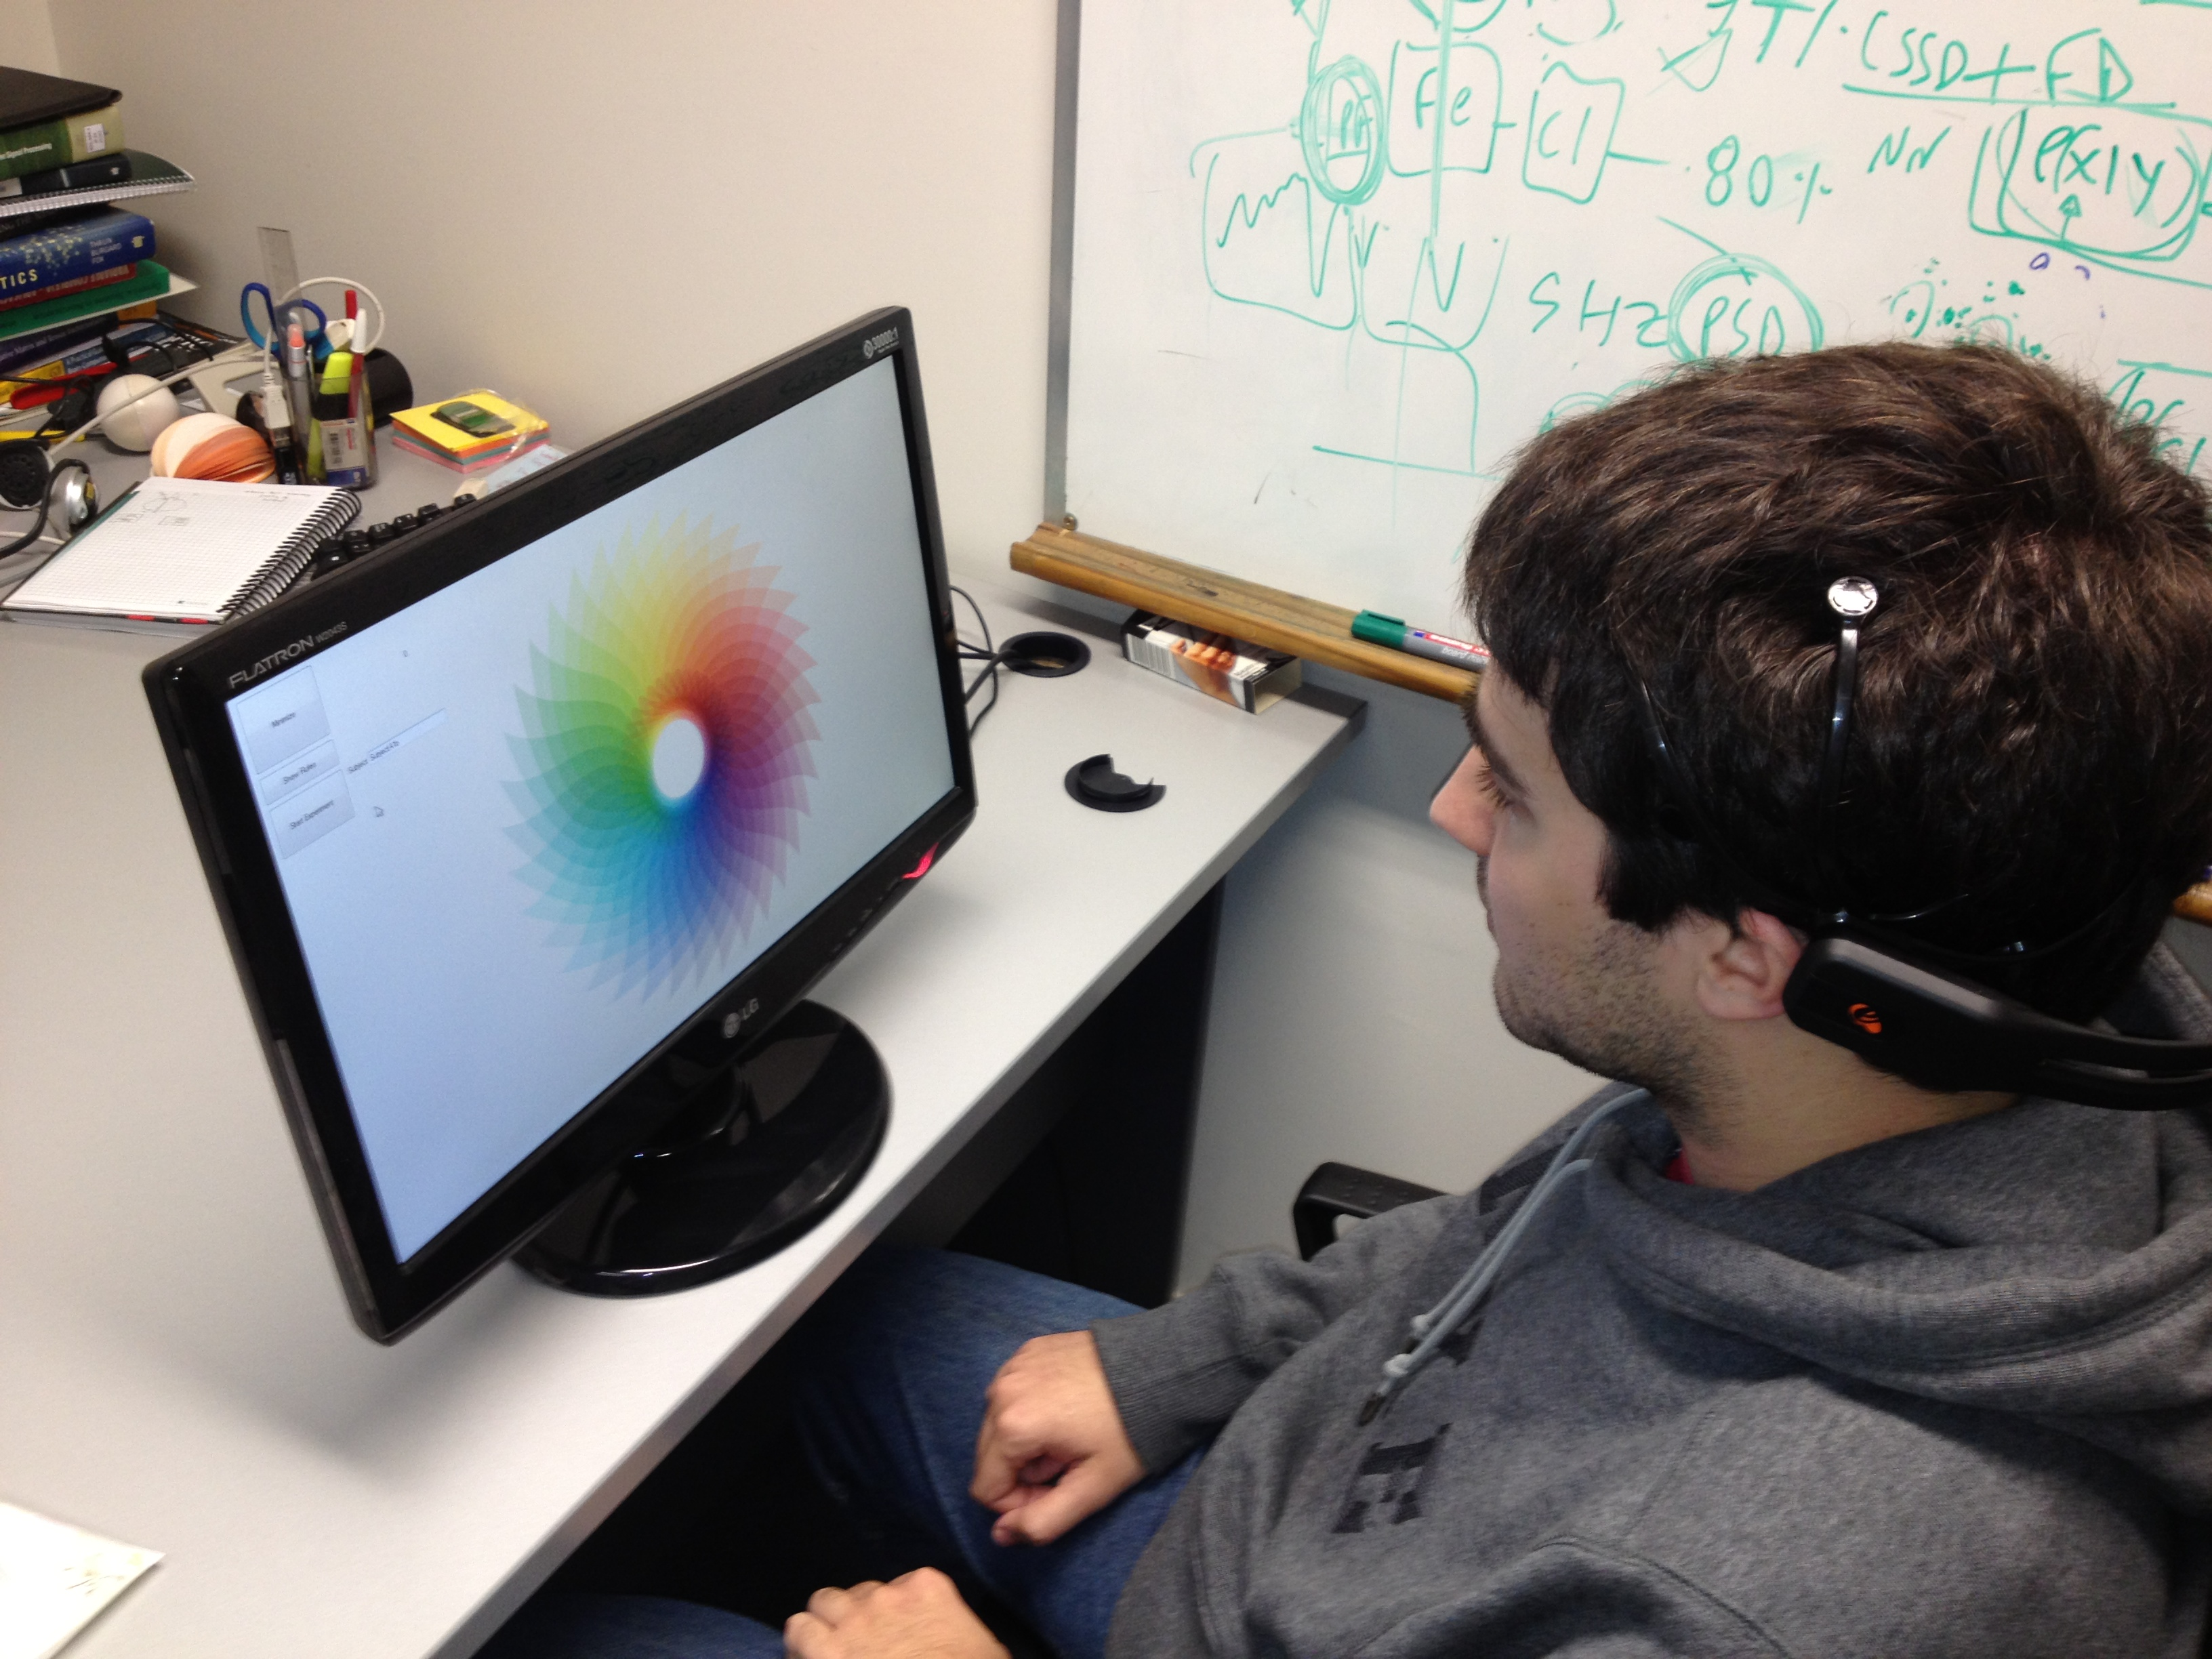
\includegraphics[width=3.5cm, height=3cm]{images/emotivdatasetsubject.jpg}}
\caption[EPOC Emotiv Alpha Waves Dataset]{(a)EPOC Emotiv consumer-grade 14-channels Wireless EEG.(b) This device has a fixed set of positions according to the 10-20 International System.(c) While resting and sitting confortable in a chair, subjects had to fixate their sight to the center of this image which was being displayed on a computer monitor, 1 \si{meter} away from the subject.(d) Subject performing the experiment described to produce the Dataset described in \ref{dataset1}}.
\label{fig:alpharesults}
\end{figure}

      
\subsection{Dataset II - AlphaNet Dataset}
Additionally, the performance of HIST was tested against the public dataset EEG Motor Movement/Imagery Dataset of the PhysioNet effort published and mantained by the NHS~\cite{Schalk2004,Goldberger2000}.  

Baseline records and motor/imagery tasks were performed by 109 healthy volunteers, using the BCI2000 system~\cite{Schalk2004}.  At the same time 64-channel EEG records were registered where each subject completed 14 tasks, called Runs.  The first two are the baseline calibration tasks, of relevance for this Chapter.  These Runs 1 and 2 are each one-minute records of resting subjects with eyes open and eyes closed.  From these records, 60 segments of 1-second length are further extracted per subject. Class labeling is the same as Dataset I.  The experiment was performed on 25 of the 109 subjects.


%This dataset
%
%Subjects performed different motor/imagery tasks while 64-channel EEG were recorded using the BCI2000 system (http://www.bci2000.org). Each subject performed 14 experimental runs: two one-minute baseline runs (one with eyes open, one with eyes closed), and three two-minute runs of each of the four following tasks:
%
%A target appears on either the left or the right side of the screen. The subject opens and closes the corresponding fist until the target disappears. Then the subject relaxes.
%A target appears on either the left or the right side of the screen. The subject imagines opening and closing the corresponding fist until the target disappears. Then the subject relaxes.
%A target appears on either the top or the bottom of the screen. The subject opens and closes either both fists (if the target is on top) or both feet (if the target is on the bottom) until the target disappears. Then the subject relaxes.
%A target appears on either the top or the bottom of the screen. The subject imagines opening and closing either both fists (if the target is on top) or both feet (if the target is on the bottom) until the target disappears. Then the subject relaxes.


\subsection{Parameters}

Descriptors are extracted from all the generated images, from both classes, and they are used to classify images in a 10-fold cross-validation procedure.
Keypoint localization is determined according to Section~\ref{keypointlocation} by following the trace of the signal, with a $\gls{kpd} = 1$.  The NBNN classification method described in Section~\ref{nbnn} is used.  The parameter $\gls{gamma}$ is set to $1$, as well as $\gls{gammat}$.  

%For the first two datasets, as the sampling frequency of both datasets is similar, Image and SIFT Descriptor Scale were adjusted to delta and gamma to 1.

%\subsection{Dataset III - BCI Competition 2003 IV \textit{self-paced 1s}}
%We validated our method against the "BCI Competition 2003, dataset IV \textit{self-paced 1s}" \cite{c51}. This dataset is composed of 28 channels, in 416 epochs of 50 samples per epoch (500 ms length at 100 Hz) each one with the corresponding label, where subjects were asked to type at will a letter on a keyboard with the right or left index finger.  It is based on the Bereitschaftspotential \cite{c52}, which is a Slow Cortical Potential, particularly a slow change in voltages towards a negative potential drift, around 1000-500 ms before the onset of the self-initiated movement.  In this case, the information lies strongly on the time-domain.
%
%This dataset was recorded from a healthy subject during a no-feedback session. She/he sat in a normal chair with relaxed arms resting on the table and fingers in the standard typing position at the computer keyboard. The task was to press with the index and little fingers the corresponding keys in a self-chosen order and timing 'self-paced key typing'. The experiment consisted of 3 sessions of 6 minutes each. All sessions were conducted on the same day with some minutes break in-between. Typing was done at an average speed of 1 key per second.  

\section{Results}

Dataset I was controlled and verified by processing it with a 8-12Hz band-pass filter, and calculating the average power spectral density across subjects for each channels.  It can be observed on Figure \ref{fig:psd}(a)  that values corresponding to class 2 (eyes closed) are always higher than the values obtained for class 1 (eyes open). On the other hand, for the sake of illustration, a scatter plot of the obtained segment's PSD for O1 vs O2 for Subject 2 is shown, where a clear separation of classes can be devised.  In brief, there is discriminative information in the frequency-domain.



\begin{figure}[h!]
\centering
\subfigure[PSD averaged across 10 subjects for each channel. Values for Class 2 (red) are always higher than values for Class 1 (blue).]
{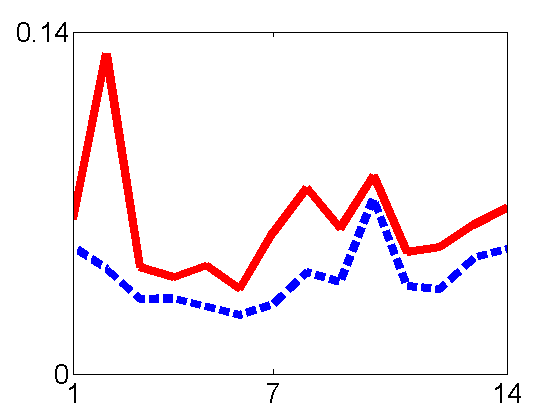
\includegraphics[width=7.5cm, height=5cm]{images/PSDExperiment1VsExperiment5.png}}
\subfigure[Scatterplot of PSD for the channel O1 vs O2.  There is a separation of classes between the red (class 2) and blue(Class 1) dots.]
{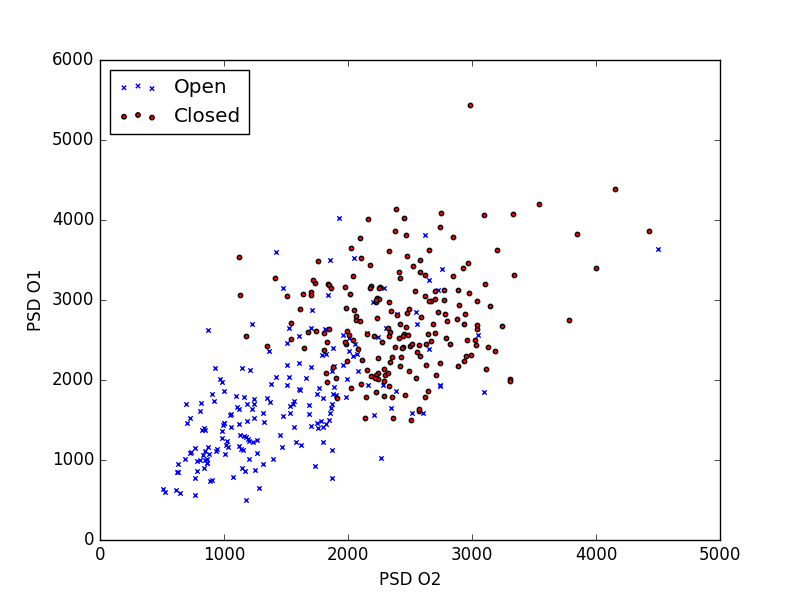
\includegraphics[width=7.5cm, height=5cm]{images/alphawavesscatterpsd.png}}
\caption[Power Spectral Density of the Dataset I]{Verification and control of the obtained Dataset I.}
\label{fig:psd}
\end{figure}
   
Results of applying a 10-Fold Cross Validation procedure on the entire set of labeled descriptors is shown on Figure~\ref{fig:alpharesultsdataseti}.  Descriptors from different subjects were used as part of the different training set to classify unknown images, so the obtained accuracy level was subject-independent.  Moreover, a classification level with average above $70\%$ was obtained in Occipital channels.
   
\begin{figure}[h!]
\centering
\subfigure[10-Fold Cross-validated accuracy values for 10 subjects.  Descriptors were mixed for all the subjects.]
{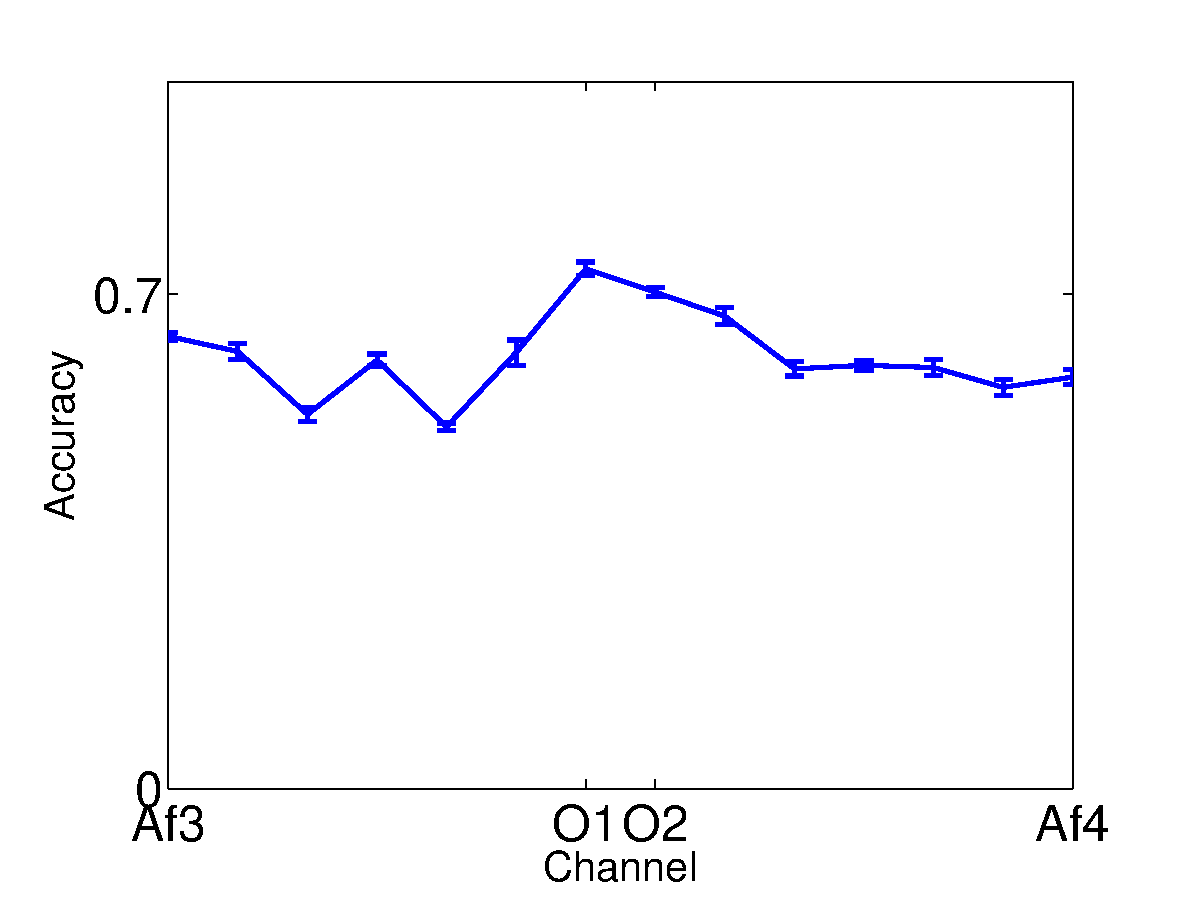
\includegraphics[width=7.5cm, height=5cm]{images/Dataset1AccuracyPerChannel}}
\subfigure[Sample Descriptor patch located on one of the images generated for one 1-second long segment of this Dataset.]
{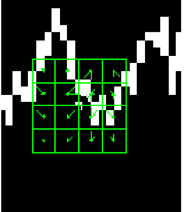
\includegraphics[width=7.5cm, height=5cm]{images/AlphaWaveSampleEEG.png}}
\caption[Dataset I Classification Rate]{The classification accuracy is maximum on occipital channels O1 and O2. The descriptor size is 12x12 pixels which corresponds to a variation of $\gls{DeltamuV} = 12$ microvolts in the signal amplitude during $\gls{lambda}=0.09$ $\si{seconds}$.}
\label{fig:alpharesultsdataseti}
\end{figure}

% Hay que traducir todo eso a los nuevos simbolos.
   

%  \begin{figure}[thpb]
%      \centering
%      \setlength\fboxsep{0pt}
%	  \setlength\fboxrule{0.5pt}
%      \fbox{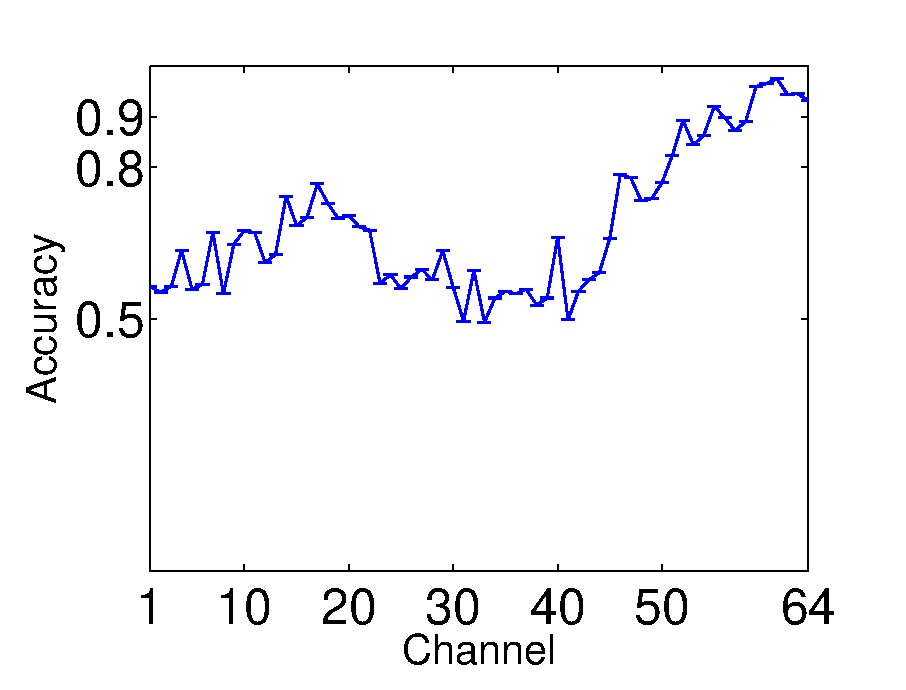
\includegraphics[width=7.5cm, height=5cm]{images/DatasetPhysionetAccuracyPerChannel}}
%      \fbox{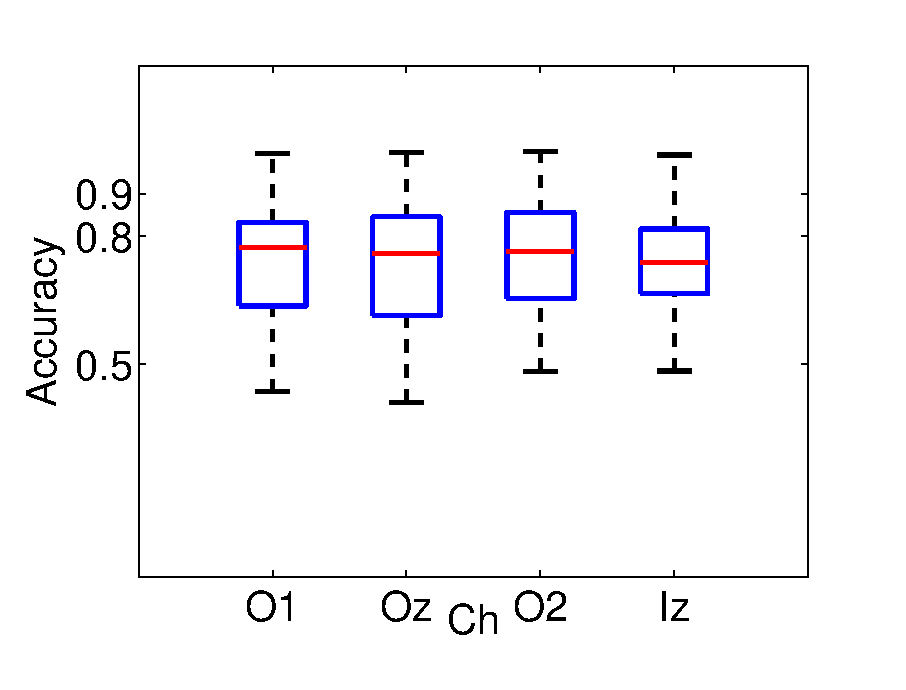
\includegraphics[width=7.5cm, height=5cm]{images/DatasetPhysionetBoxPlots}}
%      \caption[Classification Accuracy of Alpha Waves]{}
%      \label{figure1}
%   \end{figure}   
   
\begin{figure}[h!]
\centering
\subfigure[10-Fold Cross-validated accuracies for O1, Oz, O2 and Iz channels for 25 subjects of the Alphanet Dataset. Medians are above $75\%$.]
{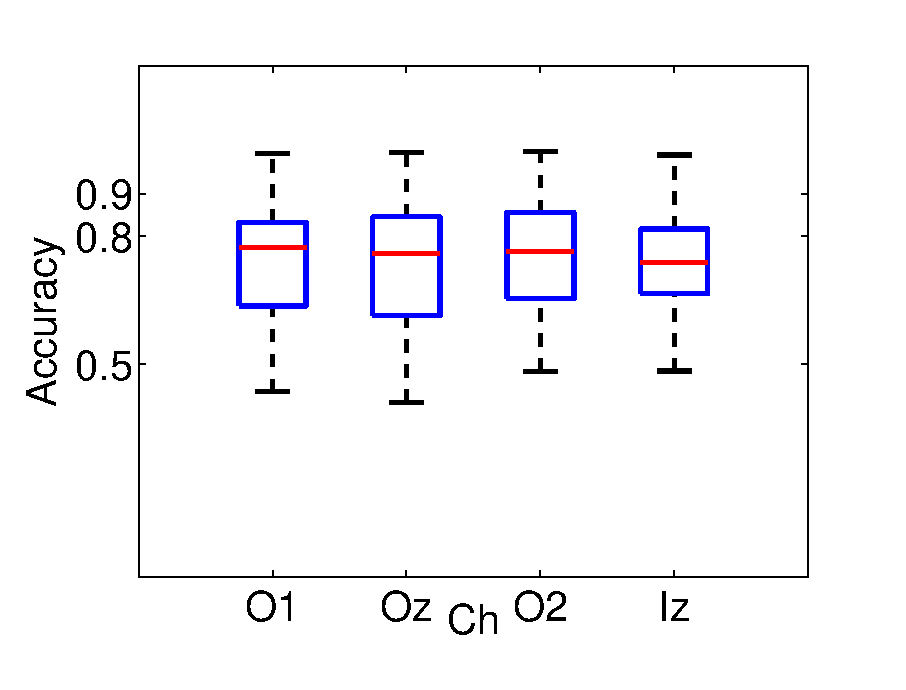
\includegraphics[width=7.5cm, height=5cm]{images/DatasetPhysionetBoxPlots}}
\subfigure[10-Fold Cross-validated accuracies values for subject number 12, using Runs 1 and 2 of the Alphanet Dataset.]
{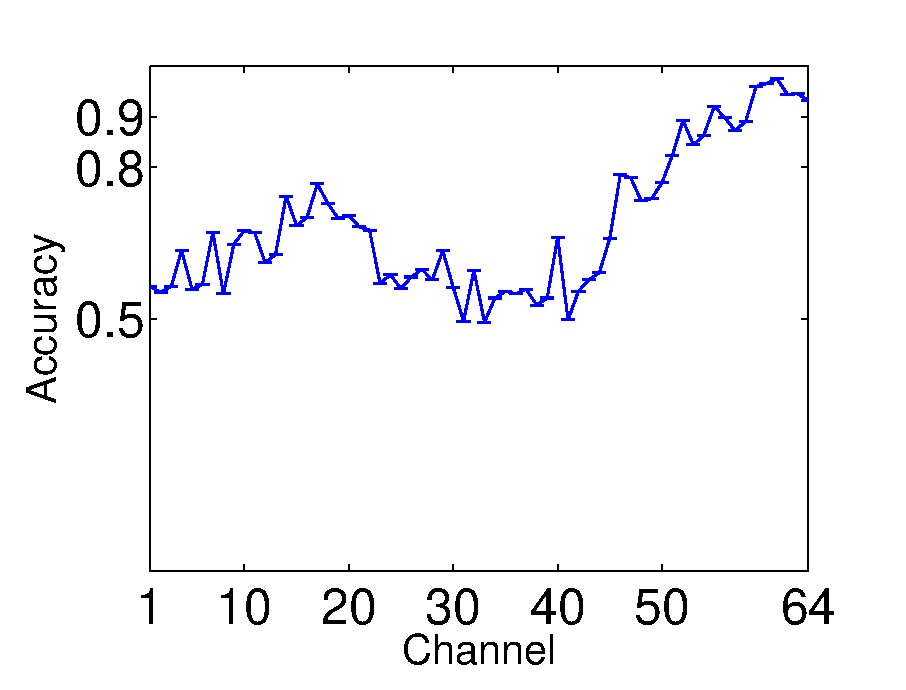
\includegraphics[width=7.5cm, height=5cm]{images/DatasetPhysionetAccuracyPerChannel}}
\caption[PhysioNet Dataset Classification Rate]{Classification Accuracy for discriminating windows of 1s ($\gls{N} = 160$) of EEG for Alpha Waves differences between subjects with eyes opened and closed.}
\label{fig:alpharesultsdatasetii}
\end{figure}


For the Dataset II, an accuracy median higher than $70\%$ for 25 subjects, also on occipital channels O1, Oz, O2 and Iz (numbered 61 to 64) is obtained while discriminating Runs 1 and 2 (Baseline eyes open vs Baseline eyes closed).  This information can be devised on Figure~\ref{fig:alpharesultsdatasetii}   (a) where boxplots of the averaged classification accuracies for all the subjects are represented.  On the other hand, Figure~\ref{fig:alpharesultsdatasetii}(b) shows the 10-Fold Validated Accuracy for one random subject. A higher accuracy in the classification of the signals can also be seen over occipital channels.

\section{Conclusion}

It is known and it was verified here that the discriminative information in EEG alpha waves is mostly contained in the frequency-domain.  In spite of this,  there is enough discriminative information to classify alpha waves signals solely on the information contained on the wiggles of the plot that is captured by the HIST method presented in this Thesis.  Offline Alpha Waves presence was detected from plots of single segments of EEG signals with an accuracy level 10-fold cross validated of 70\%.

It was also showed and proved here that there is information within the plot of a signal related to 8-12 Hz oscillatory alpha waves is higher around the occipital region and that an automated procedure which analyze visually the image structure can detect them. This important oscillatory rhythm has many connections with shifting of attention and with volitional changes and is of quite relevance in BCI research.  Particularly, the BCI paradigm of Covert Spatial Visual Attention is a further area of research for this method due to the fact that it is entirely based on analyzing alpha waves. Moreover, the posterior rythm has many implications outside the field of BCI and is very important to assess healthy EEG patterns. The exact meaning of alpha waves is still debated\cite{Ahn2013} and this basic procedure can open the possibility to explore it under a different perspective and verify if they can be effectively tied to some unexpected form of volitional control which may be effective for BCI understanding and improvement.

%The key here is the classification algorithm that was used across this thesis.  This is because the local information obtained from each descriptor "help" to balance a tendency of how the synchronous waves all behave, and that information get loaded into the class structure that is later exploited by the classification method.
%
%This results was surprassing.  We are using a method which is based on the waveform do detect a process which happens to be more prominent in spectrum.  But this shows at the same time the complex relationshipt between time and frequency.  The shape in time of a an oscilatory process prominent in frequency is clearly evident.  This goes in line with the fact that alpha waves can be seen in the EEG, and are basic tools of clinical diagnosis.

%Although EPOC Emotiv is a commercial device, more apt as HCI tool, it is possible to detect fairly some BCI components.




